%!TEX root = thesis.tex

\chapter{Evaluation}
\label{ch:evaluation}
\todo{Lee-Paper: MinMax requires simulation}

\section{Challenges for evaluation}
\label{sec:eval-challenges}

Different researchers use different metrics to evaluate the performance of their agents. 
There are multiple factors that increase the difficulty of properly evaluating the performance.

\subsection{Randomness of battles}
\label{sec:eval-challenges-randomness}
As teams are generated random, one player often ends up with a slightly better team than his opponent.
In very extreme cases, one player may not even have a chance at winning the battle. While battling
our agent during the evaluation process, one particular game stood out as the first Pokémon of 
Player one was capable of defeating the entire enemy team. \\
The Pokémon of Player on was a \textit{Volcarona} with the following moves:
\begin{itemize}
    \item \textit{Fire Blast}, a damaging \textit{Fire}-Type move
    \item \textit{Quiver Dance}, a \textit{Bug}-Type move that boots the users \ac{SPA}, \ac{SPD} and 
    \ac{SPE} by one stage each.
    \item \textit{Bug Buzz}, a damaging \textit{Bug}-Type move
    \item \textit{Roost}, a move that restores half of the user's maximum \ac{HP}
\end{itemize}
This Pokémon was able to defeat the entire enemy team with little to no possible counter play:
The first enemy Pokémon, \textit{Leafeon}, a \textit{Grass}-Type Pokémon was killed in one hit using
\textit{Fire Blast} after damaging \textit{Volcarona} using \textit{X-Scissor}. \\
Next, \textit{Glalie}, an \textit{Ice}-Type was sent into battle. \textit{Glalie} uses his best move,
\textit{Earth Quake} which brings \textit{Volcarona} to 52\% \ac{HP}. As the enemy doesn't pressure
\textit{Glalie} much, Player1 decided to boost using \textit{Quiver Dance}. Now, \textit{Volcarona}
is faster than his enemy and kills it again in one hit using \textit{Fire Blast}. \\
Then, \textit{Mr. Mime (Galar)} is sent into battle. As he fails to pressure \textit{Volcarona} as well,
Player1 can heal his Pokémon using \textit{Roost} and further boost using \textit{Quiver Dance}. After
defeating \textit{Mr. Mime (Galar)}, \textit{Volcarona} is back to 84\% HP and boosts of 2.5 \ac{SPA},
1.5 \ac{SPD} and 2.5 \ac{SPE}. \\
Boosted this high, \textit{Volcarona} can one shot both the enemy \textit{Volcarona},
\textit{Pheromosa} and the dynamaxed \textit{Scraggy} using \textit{Fire Blast}. \\
To eliminate the impact of these very extreme cases, evaluation of agents against other agents 
should be done using multiple hundred, better thousands of games against each other.
\todo{Metrik von Markus, wie viel ist denn unfair?}

\subsection{Evaluation against baseline agents}
\label{sec:eval-challenges-baseline}
A good way to get a rough idea on how well an agent performs can be to compare it against a baseline agent.
There are two very popular baseline agents, the \textit{RandomPlayer} and the \textit{MaxDamagePlayer}.
While the \textit{RandomPlayer} always chooses either a random move or a random switch, the \textit{MaxDamagePlayer}
always picks the move with the highest base power. If no move is available, the agent will switch to a random 
Pokémon. This is roughly equal to the skill level of an inexperienced beginner human. \todo{Similar
performance here, yet getting crushed later}

\subsection{Evaluation against human opponents}
As described in \todo{Link Showdown chapter}, Pokémon Showdown allows researchers to use bots on the
ranked ladder. 

\section{Results}
During this thesis, two different Agents were developed, \textit{HerrDonner} and \textit{HerrGewitter}.

\subsection{HerrDonner}
This agent was designed to establish a good baseline and to demonstrate the capabilities of a very
simple rule set. The agent is capable of looking multiple turns into the future. In order to determine
what moves to be used, the Agent generates every possible move combination with the specified amount
of turns into the future and calculates the expected outcome while assuming that the enemy does 
not move at all, similar to the \ac{BFS}-based algorithm described in paragraph \ref{sec:showdown-competition-bfs}. 
No drawback moves that heal the agent, set hazards or field conditions or inflict status conditions
are not considered unless they result in the highest amount of damage dealt. Also, stat changes are 
not taken into account, neither for damage calculation nor for determination of matchups. 
This results in the bot often spamming moves like \textit{Draco Meteor}, a \textit{special} 
\textit{Dragon}-type move that deals a lot of damage but also lowers the
users \ac{SPA} by two stages resulting in the move dealing less damage every time it is used. 
When the agent is forced to switch, it will switch to a check if available. If no check is available,
a counter is sent into battle if one exists. Otherwise, a random Pokémon will be picked. \\
At the start of each turn, \textit{HerrDonner} will check if the current matchup is not favorable, 
a matchup is deemed unfavorable, if the current Pokémon is neither \textit{check} nor 
\textit{counter} to the current enemy. On a bad matchup, the bot will switch to an available 
\textit{check} or \textit{counter}. If neither is available, the bot won't switch and try to
defeat the current opponent with his active team member. \\
Dynamaxing is implemented in a very simple and naive way: The agent will always dynamax the
active Pokémon as soon as more than four enemy Pokémon are known. Lastly, if the
current Pokémon is dynamaxed, the agent will not switch, even if the current matchup is not
favorable. 

\subsection{HerrGewitter}
\textit{HerrGewitter} behaves like described in section \ref{ch:approach}. Here, the most notable
differences between both agents are highlighted, and limitations of this agent are discussed. \\
Firstly, more things are taken into consideration when calculating damage, current stat changes are
taken into consideration as well as status conditions. In addition to that, abilities and items
are considered for damage calculation. Furthermore, recoil from moves, healing both from items
like \textit{Leftovers} \cite{Bulbapedia:Leftovers} and moves like \textit{Recover} aren't neglected
anymore. \\
Switching and the selection of moves is done as described in \ref{ch:approach}. \\
These improvements lead to \textit{HerrGewitter} avoiding mistakes of \textit{HerrDonner}. For example,
this agent will burn a physical attacker using for example \textit{Will-O-Wisp} \cite{Bulbapedia:Will-O-Wisp}
in order to reduce damage taken over the next turns. The agent will also boost and heal itself in favorable
situations which stalls the game and forces the opponent to react. Another major improvement is that the
agent switches out the current Pokémon if stat changes resulted in an unfavorable matchup which is especially
important as stat changes reset on swap. \\
There are still a lot of features that \textit{HerrGewitter} is lacking. 

\paragraph{Weather and Field effects}
The first thing to improve in future versions is to add proper support for weather and field effects in 
the damage calculator as well as in the \textit{MinMax}-Algorithm. Currently, the agent is for example
not aware of the fact that a \textit{Fire}-Type move deals 1.5 more damage during \textit{Harsh Sunlight}.

\paragraph{Hazards}
Currently, the agent will always try to set a non-present Hazard in the early game as this does most 
of the time result in a long term benefit. There are however some notable exceptions to this that 
are not yet implemented:
\begin{itemize}
  \item The agent will always set as many hazards as possible in the early game, even if the current matchup 
  is unfavorable, including always setting up to two layers of spikes. A small test on human players indicated
  that this leads to slightly better results than only setting hazards on good matchups, but due to the very
  small sample size, future work is needed to determine the best strategy for setting hazards.
  \item The agent does not take the damage taken by hazards into account when switching Pokémon. 
  \item The agent will always use \textit{Toxic Spikes} even if the opponent has a \textit{Poison}-Type
  Pokémon on his team that will remove this hazard upon being switched in.
  \item The agent will use Hazards even if the current enemy is known to have a hazard-clearing move like
  \textit{Defog} \cite{Bulbapedia:Defog}
  \item The agent will not clear hazards
\end{itemize}


\paragraph{Choice Items}
As described in section \ref{sec:Important-items} Pokémon holding a \textit{Choice}-item are locked into using always 
the same move until they are switched out. \todo{Continue here}

\paragraph{MinMax}
\todo{Boosts / Status not taken into consideration in MinMax}
\todo{Hazard damage on field enter}
\todo{Weakness: Choice Items}
\todo{Special Moves like counter }

\begin{table}[h]
    \centering
    \begin{tabular}{|l|l|l|}
    \hline 
    \textbf{Opponent}      & Wins & Losses \\
    \hline 
    \emph{RandomPlayer}    & 992  & 8      \\
    \hline 
    \emph{MaxDamagePlayer} &      &        \\
    \hline 
    \emph{HerrGewitter}    &      &        \\
    \hline 
    \end{tabular}
    \caption{Results of HerrDonner}
    \label{tab:HerrDonner}
\end{table}
\begin{table}[h]
    \centering
    \begin{tabular}{|l|l|l|}
    \hline 
    \textbf{Opponent}      & Wins   & Losses \\
    \hline 
    \emph{RandomPlayer}    & 993    & 7 \\
    \hline 
    \emph{MaxDamagePlayer} &        &        \\
    \hline 
    \emph{HerrDonner}       &       &        \\
    \hline 
    \emph{Pmariglia}        & 273   & 727 \\
    \hline
    \end{tabular}
    \caption{Results of HerrGewitter}
    \label{tab:HerrGewitter}
\end{table}

\subsection{Comparison to other agents}

\subsection{Ranked Results}
\begin{figure}[h]
    \centering
    \begin{minipage}{.5\textwidth}
      \centering
      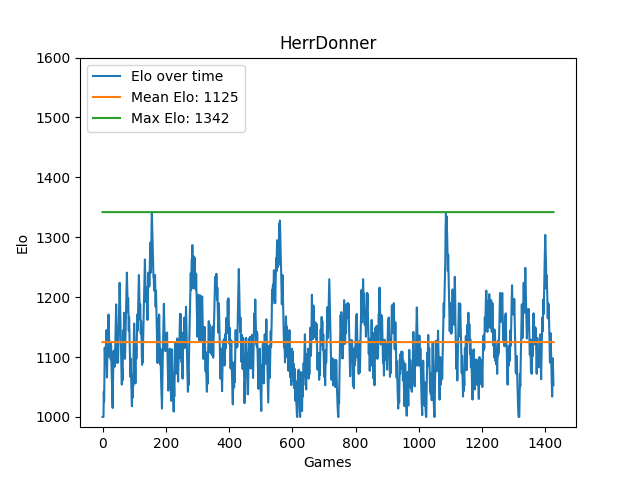
\includegraphics[width=1\linewidth]{images/Donner-Elo-Time.png}
      \captionof{figure}{Elo HerrDonner}
      \label{fig:donner-elo}
    \end{minipage}%
    \begin{minipage}{.5\textwidth}
      \centering
      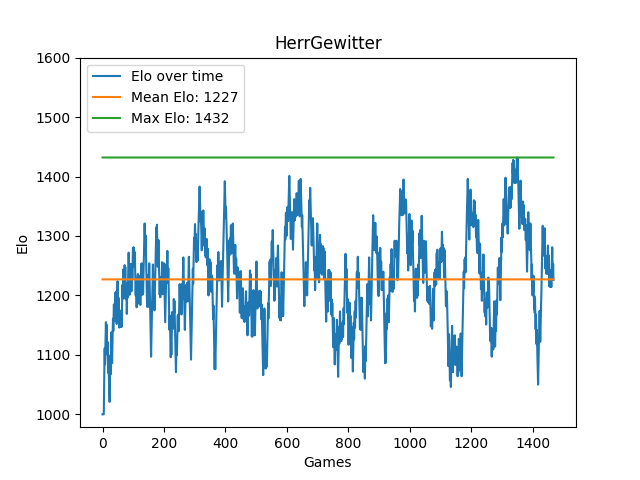
\includegraphics[width=1\linewidth]{images/Gewitter-Elo-Time.png}
      \captionof{figure}{Elo HerrGewitter}
      \label{fig:gewitter-elo}
    \end{minipage}
\end{figure}
    
\begin{figure}[h]
	\centering
	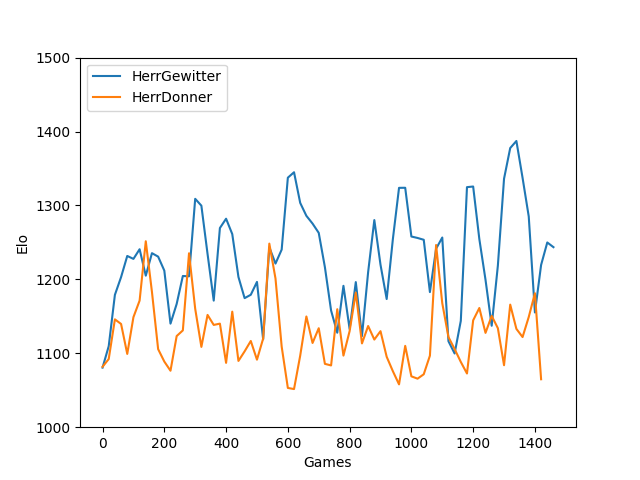
\includegraphics[width=0.7\textwidth]{images/Smoothed-Elo-Time.png}
	\caption{Smoothed Elo}
	\label{fig:elo-smoothed}
\end{figure}
 